

\begin{frame}{The Instrument Across Brazil}
\hypertarget{src:instrumentmap}{}
\footnotesize
\begin{columns}[T]
\begin{column}{0.58\textwidth}
  \centering
  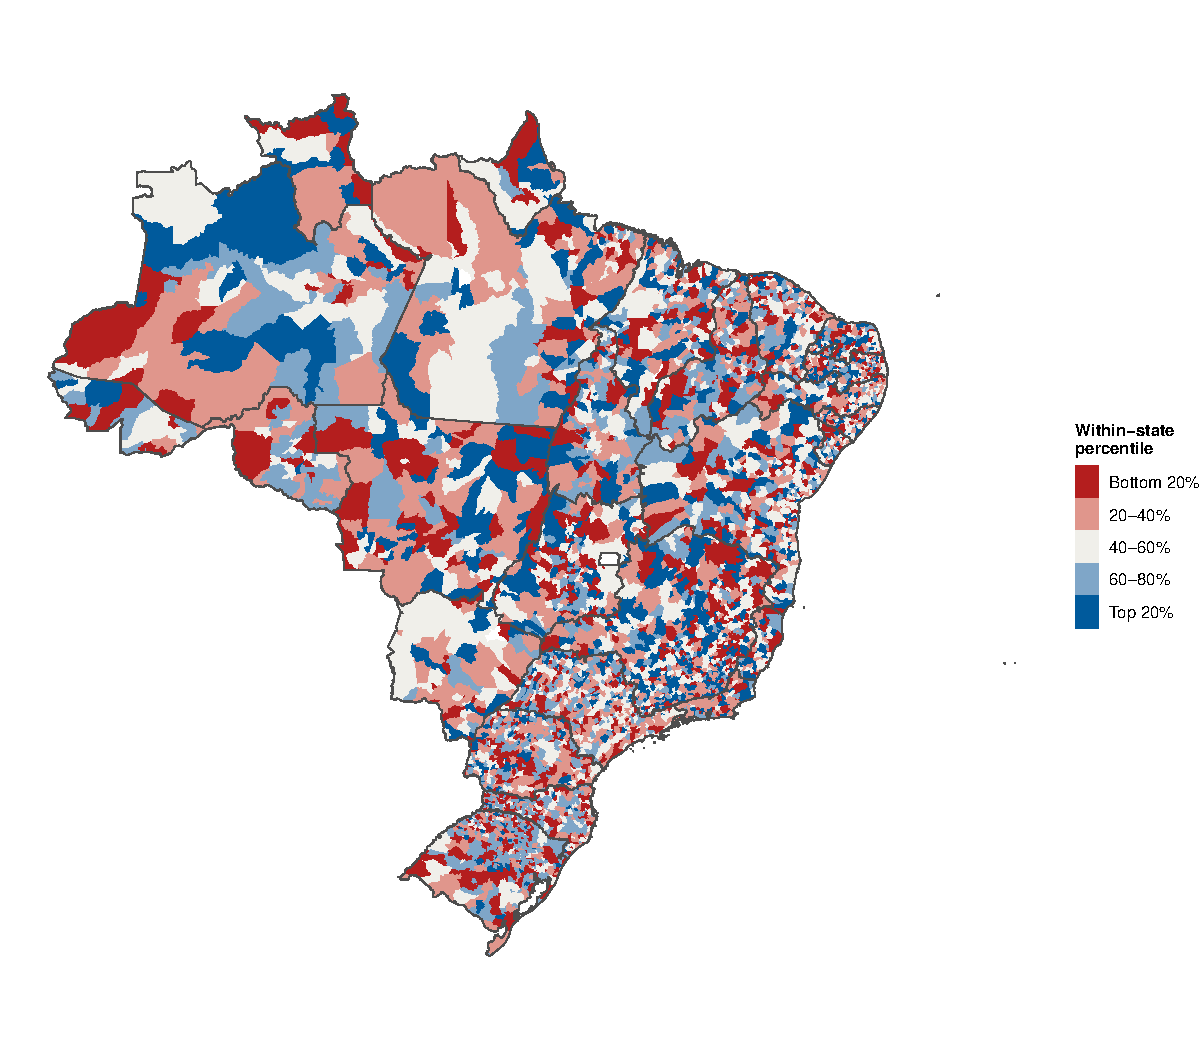
\includegraphics[width=\linewidth,height=0.60\textheight,keepaspectratio]{../figures/instrument_map.pdf}\\[4pt]
  {\scriptsize\ns{Predicted exposure by municipality. \textcolor{myblue}{Blue} = above-average, \textcolor{myred}{red} = below-average.}}
\end{column}
\begin{column}{0.40\textwidth}
  \centering
  \vspace{0.06\textheight}
  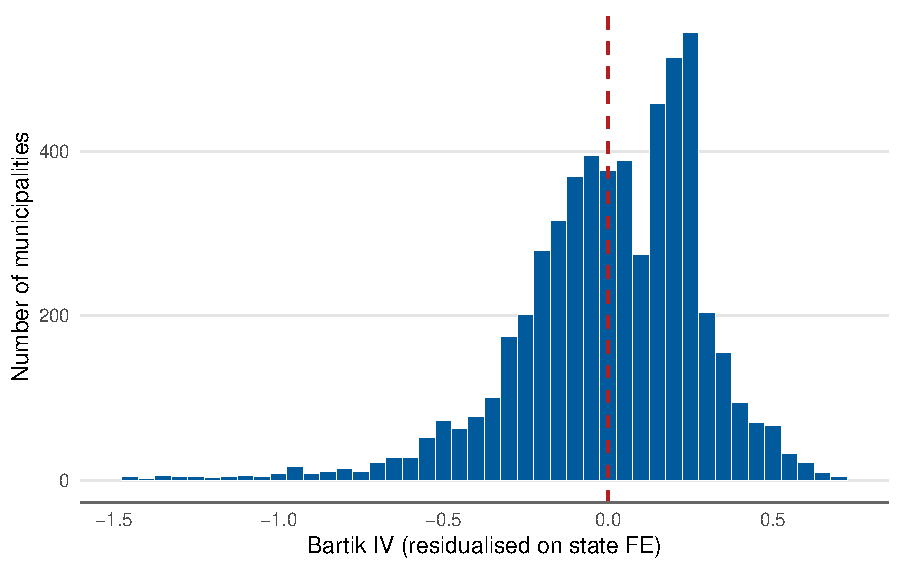
\includegraphics[width=\linewidth,height=0.42\textheight,keepaspectratio]{../figures/instrument_histogram.pdf}\\[4pt]
  {\scriptsize\ns{Instrument after removing state fixed effects. Identifying variation is \textbf{within-state} (SD $=\BartikZSDResid$).}}\\[10pt]
  \raggedright\scriptsize A heavier campaign-conduct / information-environment mix in 2020 means higher predicted litigation exposure by 2024.
\end{column}
\end{columns}
\end{frame}
